\makeatletter
\def\input@path{{../../}}
\makeatother
\documentclass[../../main.tex]{subfiles}

\graphicspath{
	{../../img/}
	{../img/}
	{img/}
}

\begin{document}
\section{Сходимость комплексных последовательностей (КП)}

Произвольное отображение
\begin{equation}\label{24:1}
f: \N \to \C
\end{equation}
называется \emph{комплексной последовательностью} (КП).

В $ \eqref{24:1} \quad \forall n \in \N \quad \exists!\, z_n = f(n) \in \C 
$.

По аналогии с действительными последовательностями будем использовать запись $ 
(z_n),\ n \in \N $.

Будем говорить, что $ (z_n) $ сходится, если
\begin{equation}\label{24:2}
	\exists\, p \in \C :\, \forall \eps > 0\quad \exists \nu = \nu_\eps \in \R 
	\quad 
	\forall n \geq \nu \implies |z_n - p| \leq \eps.
\end{equation}

Представим $ z_n $ в виде $x_n + i y_n$, где
$\begin{cases}
x_n = \Re z_n \in \R \\
y_n = \Im z_n \in \R;
\end{cases}.$

Предположим $ p = p_1 + i p_2,\ p_1, p_2 \in \R $. Тогда в силу $ \eqref{24:2} 
$ имеем:

\begin{equation}\label{24:3}
	|z_n - p| = |(x_n - p_1) + i(y_n - p_2)| = \sqrt{(x_n - p_1)^2 + (y_n - 
	p_2)^2} \leq \eps.
\end{equation}

\begin{thm}(Критерий сходимости комплексной последовательности(КП))
	\begin{equation}\label{24:4}
		z_n = x_n + i y_n \appr{n \rightarrow \infty} p = p_1 + i p_2 \iff
	\end{equation}
	\begin{equation}\label{24:5}
		\iff
		\begin{cases}
			x_n \appr{n \rightarrow \infty} p_1, \\
			y_n \appr{n \rightarrow \infty} p_2.
		\end{cases}
	\end{equation}
\end{thm}
\begin{proof}
\;

	\nec: Пусть выполнено $ \eqref{24:4} $. Тогда учитывая, что
	\[|x_n - p_1| \leq \sqrt{(x_n - p_1)^2 + (y_n - p_2)^2} = |z_n - p|,\]
	\[|y_n - p_2| \leq \sqrt{(x_n - p_1)^2 + (y_n - p_2)^2} = |z_n - p|,\]
	в силу $ \eqref{24:2}, \eqref{24:3} $, получаем:	
	\[\forall \eps > 0\quad \exists \nu \in \R\quad \forall n \geq \nu \implies 
	\begin{cases}
		|x_n - p_1| \leq |z_n - p| \leq \eps \\
		|y_n - p_2| \leq |z_n - p| \leq \eps \\
	\end{cases} \implies  \eqref{24:5}. \]
	
	\suff: Пусть выполнено $ \eqref{24:5} $. Тогда в силу  M-леммы сходимости 
	действительных числовых последовательностей имеем:
	
	\[\forall \eps > 0 \quad \exists\,\widetilde{\nu} = \widetilde{\nu}_\eps \in 
	\R\quad \forall n \geq \widetilde{\nu} \implies 
	|x_n - p_1| \leq \frac{\eps}{\sqrt{2}}\]
	
	\[\forall \eps > 0\quad \exists\,\overline{\nu} = \overline{\nu}_\eps \in 
	\R\quad 
	\forall n \geq \overline{\nu} \implies 
	|y_n - p_2| \leq \frac{\eps}{\sqrt{2}} \]
	
	Выберем $ \nu = \max\{\widetilde{\nu}, \overline{\nu}\} \in \R $. Тогда:
	\[\forall n \geq \nu \implies 
	|z_n - p| \stackrel{\eqref{24:3}}{=} \sqrt{(x_n - p_1)^2 + (y_n - p_2)^2} 
	\leq \sqrt{\left(\frac{\eps}{\sqrt{2}}\right)^2 + 
	\left(\frac{\eps}{\sqrt{2}}\right)^2} = \eps \implies \eqref{24:2}. \qedhere\]
\end{proof}

\begin{rem}
	Доказанный критерий сводит исследование сходимости комплексных
	 последовательностей к исследованию на сходимость двух действительных
	 последовательностей, состоящих соответственно из действительной и мнимой
	 частей исходной последовательности.
	
	Поэтому большинство свойств сходимости действительных последовательностей 
	 переносится на комплексные (кроме свойств с неравенствами, так как множество
	 комплексных чисел нельзя упорядочить). В связи с этим имеем:
\end{rem}
	\begin{thm}(Критерий Коши сходимости комплексных последовательностей (КП))
		$ (z_n) $ сходится $ \iff \forall \eps > 0\quad \exists \nu = \nu_\eps 
		\in \R \quad \forall\, m, n \geq \nu_\eps \implies |z_m - z_n| \leq \eps.$
	\end{thm} 

	\begin{thm}(Принцип выбора для комплексных последовательностей (КП))		
		Из любой ограниченноой последовательности $ z_n $, для которой $ \exists M = 
		const \geq 0 \quad |z_n| \leq M\quad \forall n \in \N $, можно выбрать 
		сходящуюся 
		подпоследовательность.
	\end{thm}
	
		Доказательство, в отличие от действительного случая, где используется 
		неравенство, проводится как в $n$-\text{мерных} последовательностях, без 
		сравнения.

	\begin{thm}(Арифметические операции для сходящихся КП)
		\begin{enumerate}
			\item Если $ (z_n) $ и $ (w_n) $ ~--- сходящиеся КП, то \[ \forall\, 
			\lambda, \mu \in \C \implies
			\exists\, \underset{n \to \infty}{\lim} (\lambda z_n + \mu w_n) = 
			(\lambda \underset{n \to \infty}{\lim}z_n + \mu \underset{n \to 
			\infty}{\lim}w_n) \in \R. \]
			
			\item $ \underset{n \to \infty}{\lim} (z_n \cdot w_n) = \left(\underset{n 
			\to 
			\infty}{\lim} z_n\right)\cdot\left(\underset{n \to \infty}{\lim} 
			w_n\right).$
			
			\item Если $ w_n \neq 0 $ и $ \underset{n \to \infty}{\lim} w_n 
			\neq 0 $, то $ \underset{n \to \infty}{\lim} \dfrac{z_n}{w_n} = 
			\frac{\underset{n \to \infty}{\lim} z_n}{\underset{n \to \infty}{\lim} w_n}.
			$
		\end{enumerate}
	\end{thm}

Если $ z_n \appr{n \rightarrow \infty} 0 $, то эту КП называют 
\emph{бесконечно 
малой последовательностью} и пишут $ z_n \underset{n \to \infty}{=} o(1) $.

\begin{exc}
	По аналогии с числовыми последовательностями сформулировать основные свойства 
	комплексных бмп.
\end{exc}

\medskip

Последовательность, не являющуюся сходящейся, называют расходящейся. Среди 
расходящихся последовательностей выделяют ББП (бесконечно большие 
последовательности).
$ (z_n) $ является ББП, если $ \forall \eps > 0\quad \exists \nu = \nu_\eps 
\in 
\R\quad \forall n > \nu \implies |z_n| \geq \eps.$
При этом, в отличие от действительного случая, в КП не используются величины $ 
+\infty, -\infty $.

Как и в действительном случае, можно показать, что если $ \forall z_n \neq 
0,\ z_n = o(1) $, то $ w_n = \frac{1}{z_n} $ ~--- ББП, и наоборот.

\begin{exmp}
	\;
	\begin{enumerate}
		\item $ z_n = q^n,\ n \in \N,\ q \in \C - \fix $.
		
		\begin{enumerate}
			\item Если $ q = 0 $, то $ \forall z_n = 0 \implies z_n = o(1) $;
			
			\item Если $ 0 < |q| < 1 $, то решая неравенство $ |q|^n \leq \eps \iff 
			n \geq \log_{|q|}\eps $ получаем, что $ \forall\, \eps > 0 \quad \exists\, 
			\nu = \log_{|q|}\eps \in \R \quad \forall\, n \geq \nu \quad |q^n| = 
			|q|^n \leq |q|^\nu = \eps \implies z_n \underset{n \to \infty}{=} o(1) $.
			
			\item При $ |q| > 1 $ получаем, что \[\forall\, \eps > 0 \quad \exists\, 
			\nu = \log_{|q|}\eps \in \R: \quad \forall\, n \geq \nu \quad |z_n| = 
			|q^n| \geq [|q| > 1, n \geq \nu] \geq {|q|}^{\nu} = \eps,\] т.~е. 
			$(z_n)$~--- ББП.
			
			\item При $ q = 1 \quad \forall z_n = 1 \appr{n \rightarrow \infty} 1 \in 
			\C $ ~--- сходящаяся КП.
			
			\item Если $ |q| = 1, q \neq 1 $, то $ (z_n) $ расходится, так как в этом 
			случае $ \exists\, \phi_0 \in ]-\pi, 0[ \cup ]0, \pi] $ такое, что $ z = 
			e^{i\phi_0} = \cos{\phi_0} + i\sin{\phi_0} $ и 
			$ \begin{cases}
				\nexists \underset{n \to \infty}{\lim} \cos{n\phi_0}, \\
				\nexists \underset{n \to \infty}{\lim} \sin{n\phi_0}.
			\end{cases} $
			
			Ответ: 
			$ (q^n) = \begin{cases}
				\text{бмп, если } |q| < 1 \\
				\text{ББП, если } |q| > 1 \\
				1 \text{, если } q = 1 \\
				\text{расходится, если } |q| = 1, q \neq 1
			\end{cases} $
		\end{enumerate}
	\end{enumerate}
\end{exmp}

Множество комплексных чисел $ \C $, пополненное бесконечно удаленной точкой $ 
z = \infty $, будем обозначать $ \overline{\C} = \C \cup {\infty} $.

Для графического изображения $ \overline{\C} $ используют стереографическую 
проекцию сферы Римана на плоскость. Эта стереографическая проекция дает 
взаимооднозначное соответствие между сферой Римана и комплексной плоскостью. 
Точке $ \infty $ соответствует точка $P$ сферы.

\begin{center}
	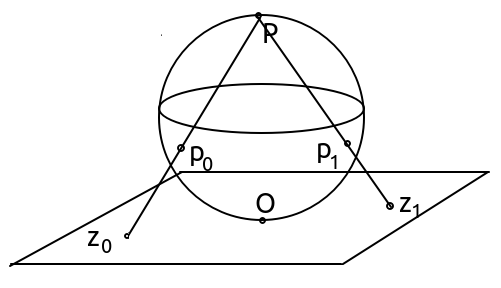
\includegraphics[scale = 0.8]{lec24_1} 
\end{center}

Указанная стереографическая проекция используется в картографии в силу того, 
что угол на север (точку $P$) будет совпадать с углом на плоскости образов 
линий. То есть, углы $\angle p_0Pp_1$ и $\angle z_0Pz_1$ совпадают.

\section{Ряды с комплексными членами}

Как и в $ \R $, для задания ряда для КП $ (z_n) $ строим последовательность 
\begin{equation}\label{24:6}
	s_n = z_1 + z_2 + \ldots + z_n,\, n \in \N
\end{equation}

Если $ \exists\, \underset{n \to \infty}{\lim} s_n = s_0 \in \C $, то в этом 
случае говорим, что имеется сходящийся ряд с комплексными членами
\begin{equation}\label{24:7}
	\sum_{k=1}^{\infty}z_k,
\end{equation}
сумма которого равна
\begin{equation}\label{24:8}
	s_0 = \underset{n \to \infty}{\lim} s_n = \underset{n \to \infty}{\lim} 
	\sum_{k=1}^{n}z_k\, \in \C.
\end{equation}

Если последовательность $ s_n $ расходится, то соответствующий ей ряд $ 
\eqref{24:7} $ также расходится. В $ \eqref{24:7}\, z_n $ ~--- общий член 
комплексного ряда (КР), а в $ \eqref{24:6}\, s_n $ ~--- последовательность 
частных сумм ряда $ \eqref{24:7} $.

\begin{exmp}(Комплексный геометрический ряд)
	\;
	
	Для $ \fix\, q \in \C $ рассмотрим $ \sum\limits_{k=1}^{\infty}q^{n - 1} = 1 
	+ q + 
	q^2 + \ldots $.
	
	Для его частных сумм имеем:
	
	\[s_n = 1 + q + q^2 + \ldots + q^{n - 1} =
	\begin{cases}
		\dfrac{1 - q^n}{1 - q},& q \neq 1 \\
		n,& q = 1
	\end{cases}\]
	
	Для $ q = 1,\ s_n \appr{n \rightarrow \infty} \infty $ получаем, что в этом 
	случае КР расходится.
	
	Если $ |q| < 1 $, то в силу предыдущего примера $ q^n \appr{n \rightarrow 
	\infty} 0 
	\implies \exists\, \underset{n \to \infty}{\lim} s_n = \dfrac{1}{1 - q} $. А 
	значит, в этом случае рассматриваемый КР сходится и 
	\[\sum_{n=1}^{\infty}q^{n - 1} \stackrel{|q| < 1}{=} \frac{1}{1 - q}.\]
	
	Если же $ |q| > 1 $, то в силу предыдущего примера $ s_n \appr{n \rightarrow 
	\infty} \infty \implies $ ряд расходится.
	
	Учитывая также, что в случае $ |q| = 1,\ q \neq 1 \implies \nexists\, s_n 
	\implies $ ряд расходится.
	
	Таким образом:
	\[\sum_{n=1}^{\infty}q^{n - 1} = 
	\begin{cases}
		\dfrac{1}{1 - q},& |q| < 1 \\
		\text{расходится},& |q| \geq 1
	\end{cases}\]
\end{exmp}

\begin{thm}(Критерий сходимости КЧР)
	\[\text{Ряд} \quad \sum_{n=1}^{\infty}z_n\, \text{сходится} \iff 
	\text{одновременно сходятся ряды} \sum_{n=1}^{\infty}\Re z_n\, \text{и}\, 
	\sum_{n=1}^{\infty}\Im z_n.\]
\end{thm}
\begin{proof}
	Доказательство следует из того, что если $z_n = x_n + iy_n$, $x_n = 
	\Re z_n$, $y_n = \Im z_n $, то для $ s_n $ имеем
	
	\[s_n = z_1 + \ldots + z_n = (x_1 + \ldots + x_n) + i(y_1 + \ldots + y_n) = 
	X_n + iY_n\]
	
	Из критерия сходимости КП получаем, что
	\[ s_n\, \text{сходится} \iff \text{сходятся}\, X_n, Y_n \iff \text{сходятся} 
	\sum_{n=1}^{\infty}\Re z_n, \quad \sum_{n=1}^{\infty}\Im z_n \qedhere\]
\end{proof}

\begin{rems}
	\begin{enumerate}
		\;
		
		\item В связи с тем, что для произвольного комплексного ряда его 
		сходимость/расходимость определяется сходимостью/расходимостью 
		действительных 
		числовых рядов из его мнимой и действительной частей, то основные свойства 
		комплексных числовых рядов можно получить из соответствующих признаков 
		действительных ЧР.
		
		\item Как и в $ \R $, определяется линейная комбинация КЧР:
		\[\lambda \sum_{n=1}^{\infty}z_n + \mu \sum_{n=1}^{\infty}w_n = 
		\sum_{n=1}^{\infty}(\lambda z_n + \mu w_n)\]
		
		При этом, если $ \sum z_n $ и $ \sum w_n $ сходятся, то их линейная 
		комбинация $ \forall\, \lambda, \mu \in \C $ также сходится.
		
		\item Как и для ЧР, определяется произведение КЧР по Коши:
		\[\left(\sum_{n=1}^{\infty}z_n\right)\left(\sum_{n=1}^{\infty}w_n\right) 
		= \sum_{n=1}^{\infty} 
		u_n, \quad u_n = z_1w_{n} + z_2w_{n - 1} + \ldots + z_nw_1 = \sum_{i + j = n 
		+ 1} z_iw_j, \quad n \in \N.\]
		
		Если ряды $ \sum z_n $ и $ \sum w_n $ сходятся абсолютно, то есть сходятся $ 
		\sum |z_n| $ и $ \sum |w_n| $, тогда их произведение по Коши будет 
		сходящимся рядом, и при этом
		\[\left(\sum_{n=1}^{\infty}z_n\right)\left(\sum_{n=1}^{\infty}w_n\right) = 
		\left(\sum_{n=1}^{\infty}u_n\right).\]
	\end{enumerate}
\end{rems}

\begin{thm}(Критерий абсолютной сходимости КЧР)
	\[\text{Ряд} \quad \sum_{n=1}^{\infty}z_n \text{ сходится абсолютно} \iff 
	\text{ряды } \sum_{n=1}^{\infty}|\Re z_n|, \sum_{n=1}^{\infty}|\Im z_n| 
	\text{ сходятся.}\]
\end{thm}
\begin{proof}
	Пусть $ z_n = x_n + iy_n, \quad x_n = \Re z_n \in \R, \quad y_n = \Im z_n \in 
	\R $.
	
	\nec: Если ряд $ \sum |z_n| $ сходится, то в силу неравенств
	\[|x_n| \leq \sqrt{x_n^2 + y_n^2} = |z_n|\]
	\[|y_n| \leq \sqrt{x_n^2 + y_n^2} = |z_n|\]
	по признаку сравнения для ЧР получаем, что сходятся ряды $ \sum |x_n| $ и $ 
	\sum |y_n| $, то есть $ \sum x_n $ и $ \sum y_n $ сходятся абсолютно.
	
	\suff: Пусть ряды $ \sum |x_n| $ и $ \sum |y_n| $ сходятся. В этом случае в 
	силу неравенства
	\[|z_n| = \sqrt{x_n^2 + y_n^2} = \sqrt{(|x_n| + |y_n|)^2 - 2|x_n||y_n|} \leq 
	\sqrt{(|x_n| + |y_n|)^2} = |x_n| + |y_n|\]
	и того, что
	\[\sum_{n=1}^{\infty}(|x_n| + |y_n|) = \sum_{n=1}^{\infty}|x_n| + 
	\sum_{n=1}^{\infty}|y_n|\]
	сходится, получаем по признаку сравнения для ЧР, что $ \sum |z_n| $ сходится, 
	то есть  $ \sum z_n $ сходится абсолютно.
\end{proof}

\begin{rem}
	Как и в $ \R $, из абсолютной сходимости КЧР всегда следует его обычная 
	сходимость. Обратное, вообще говоря, неверно.
\end{rem}

\begin{exmp}
	\;
	\begin{enumerate}
		\item Для $ \fix\, \alpha \in \R $ рассмотрим ряд $ \sum 
		\dfrac{e^{\frac{i}{n}}}{n^\alpha} $ и исследуем его на абсолютную сходимость.
		
		Для $ z_n = \frac{e^{\frac{i}{n}}}{n^\alpha}$ получаем: \[|z_n| = 
		\frac{1}{n^\alpha} |e^{\frac{i}{n}}| = \left[|e^{\frac{i}{n}}| = 
		\left|\cos\left(\frac{1}{n}\right) + i\sin\left(\frac{1}{n}\right)\right| = 
		\sqrt{\cos^2\left(\frac{1}{n}\right) + 
		\sin^2\left(\frac{1}{n}\right)} = 1\right] = \frac{1}{n^\alpha}.\]
		
		Отсюда, учитывая, что $ \sum \frac{1}{n^\alpha} $ сходится при $ \alpha > 1 
		$ и расходится при $ \alpha \leq 1 \implies $ для $ \alpha > 1 $ ряд $
		\sum z_n $ сходится абсолютно. В случае $ \alpha \leq 1 $ ряд из $ z_n $ 
		если и сходится, то только условно.
		\[x_n = \Re z_n = \frac{\cos(\frac{1}{n})}{n^\alpha}\]
		\[y_n = \Im z_n = \frac{\sin(\frac{1}{n})}{n^\alpha}\]
		\[x_n \sim \frac{1}{n^\alpha} \implies 
		\begin{cases}
			x_n \quad \text{сходится}, &\alpha > 1 \\
			x_n \quad \text{расходится}, &\alpha \leq 1
		\end{cases}\]
		
		Аналогично $\displaystyle y_n \sim \left[\sin\left(\frac{1}{n}\right) \sim 
		\frac{1}{n} = 
		\frac{1}{n^{\alpha + 1}}\right] \implies
		\begin{cases}
		y  \text{ сходится},& \alpha > 0 \\
		y_n  \text{ расходится},& \alpha \leq 0
		\end{cases} $
		
		Таким образом, если $ \alpha \leq 1 $, то хотя бы один из рядов $ x_n, y_n $ 
		расходится, а значит расходится и $ z_n $.
		
		Таким образом:
		\[ \sum_{n=1}^{\infty}\frac{e^{\frac{i}{n}}}{n^\alpha}\implies
		\begin{cases}
		\text{сходится},& \alpha > 1 \\
		\text{расходится},& \alpha \leq 1
		\end{cases}\]
		
	\item Используя произведение КЧР по Коши для $ \sum q^{n - 1} $, абсолютно 
	сходящегося при ${|q| < 1}$, имеем
	
	\[\left(\sum_{n=1}^{\infty}q^{n - 1}\right)^2 = \left(\sum_{n=1}^{\infty}q^{n 
	- 
	1}\right)\left(\sum_{n=1}^{\infty}q^{n - 1}\right) = (1 + (1 + 1)q + (1 + 1 + 
	1)q^2 + \ldots ) = \]
	\[= 1 + 2q + 3q^2 + \ldots\, \implies
	\sum_{n=1}^{\infty}nq^{n - 1} = [|q| < 1] = 
	\left(\sum_{n=1}^{\infty}q^{n}\right)^2 = 
	\frac{1}{(1 - q)^2}.\]
	\end{enumerate}
\end{exmp}

\end{document}
